After the architectural report, we took in consideration the remarks pointed by our teacher and his assistant. We updated it to correct relations between objects. \\

\subsection{UML Class diagram}

\begin{figure}[!ht]
	\begin{center}
		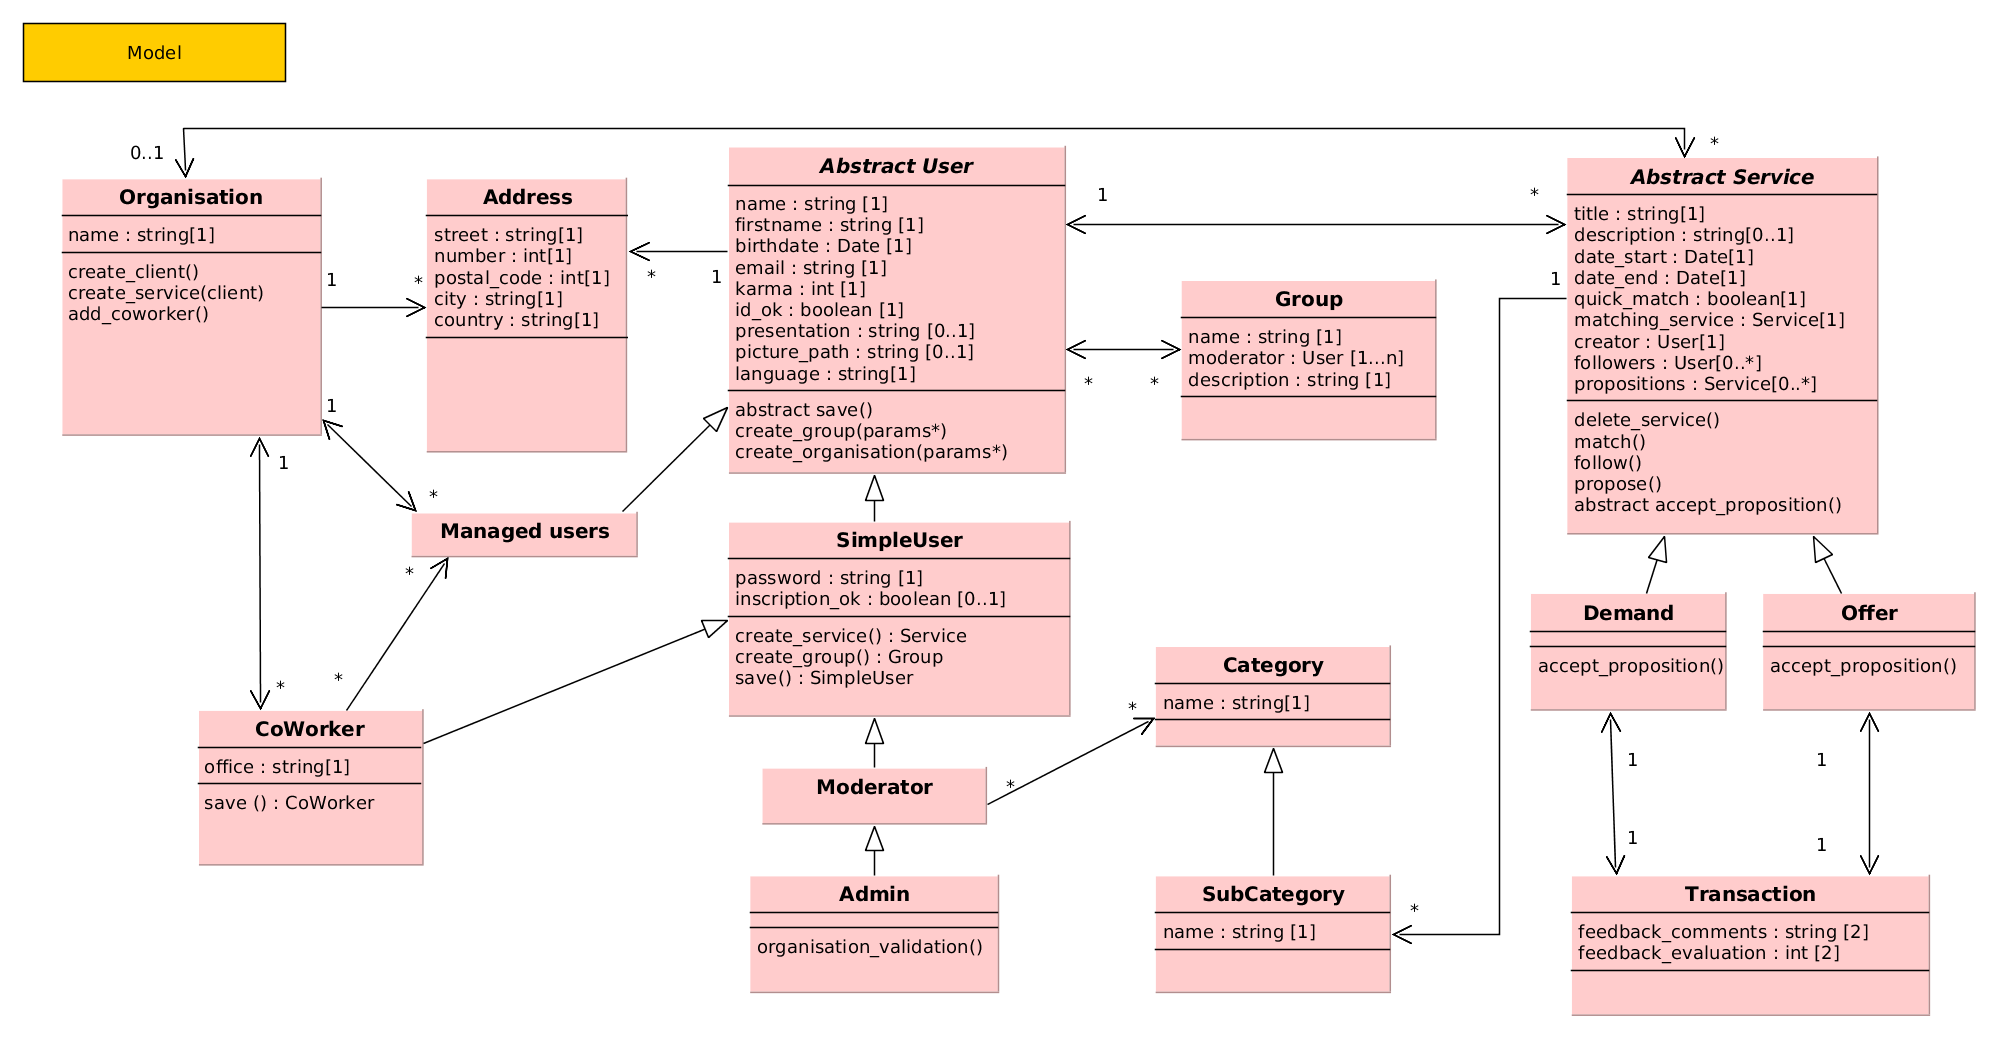
\includegraphics[width=\textwidth]{UML.png}
		\caption{Unified Modeling Language (UML): class diagram, model. This figure is also visible in a bigger size in the appendix, figure \vref{fig:uml_big}}
		\label{fig:uml}
	\end{center}
\end{figure}

Our diagram can be divided in three parts. The first part, on the left, shows the organisation part of the model. The organisation object has a name and contains some addresses (an organisation can have multiple contact points), some co-workers, managed users and created services by its users. This last link, between an organisation and a service, is absolutely not mandatory; it exists only if the service is created by a co-worker for a managed user. The co-workers are working for a single organisation for some users. They are modelled by an extension of a user because they will have an account to log in and they will be able to create services, even if it's for other users.\\

The second part, on the center of the diagram, is dedicated to the users. A main user is defined as an abstract user and contains all the informations that are in common for each kind of users. The application will be used by five kinds of users, directly or indirectly. The most common one is defined as a simple user. A user that will connect to the application from his home, sign in and he's ready to offer or demand services. This kind of account needs an e-mail verification and a password to connect to. Extension of this kind of user can be divided in two groups, the coworkers of an organisation and the administrators of the website. We already talked about coworkers a few lines above. For administrators, there are two level of responsibilities. First level is for moderators who will be able to manage services from the categories they are bound to. This choice is made to restrict responsibilities to some categories for a single administrator. The more powerful administrators stand at level 2. They are able to accept organisation registrations and manage users account (delete them if they don't respect the website policies). Notice that a user can have multiple addresses, it's a choice led by the idea of helping users to show different places where the service can be delivered. \\

The third part, on the right, explains the service part of the model. As for the users, we created an abstract part for services containing the object common parameters. A service is related to several subcategories to help user in his searches. In the same philosophy as we saw on websites like \textit{eBay}, we divided categories in subcategories. For example, a demand asking for clothes can be more detailed in specifying what kind of clothes the user wants (like winter clothes, summer clothes,etc.). Extensions of the abstract class are the specific kind of services : offers and demands. They are regrouped after a match in an object called transaction that will contains feedback from both users. You can see that we added a boolean \texttt{Quick} field in the service object. It's used to point a service that's created for a manual matching. For example, a user accepts an offer without having created a demand which match this offer. The  matching demand creation for registering the transaction in the database will not appear to the user.\\

Since we have more experiences in Java programming, we are used to design class diagrams with abstract classes. In Ruby, using abstract classes isn't as usual than in Java, and a bit harder to implement. We'll maybe define these objects as standard objects but we'll never instantiate them.\\
\begin{figure}[!ht]
	\begin{center}
		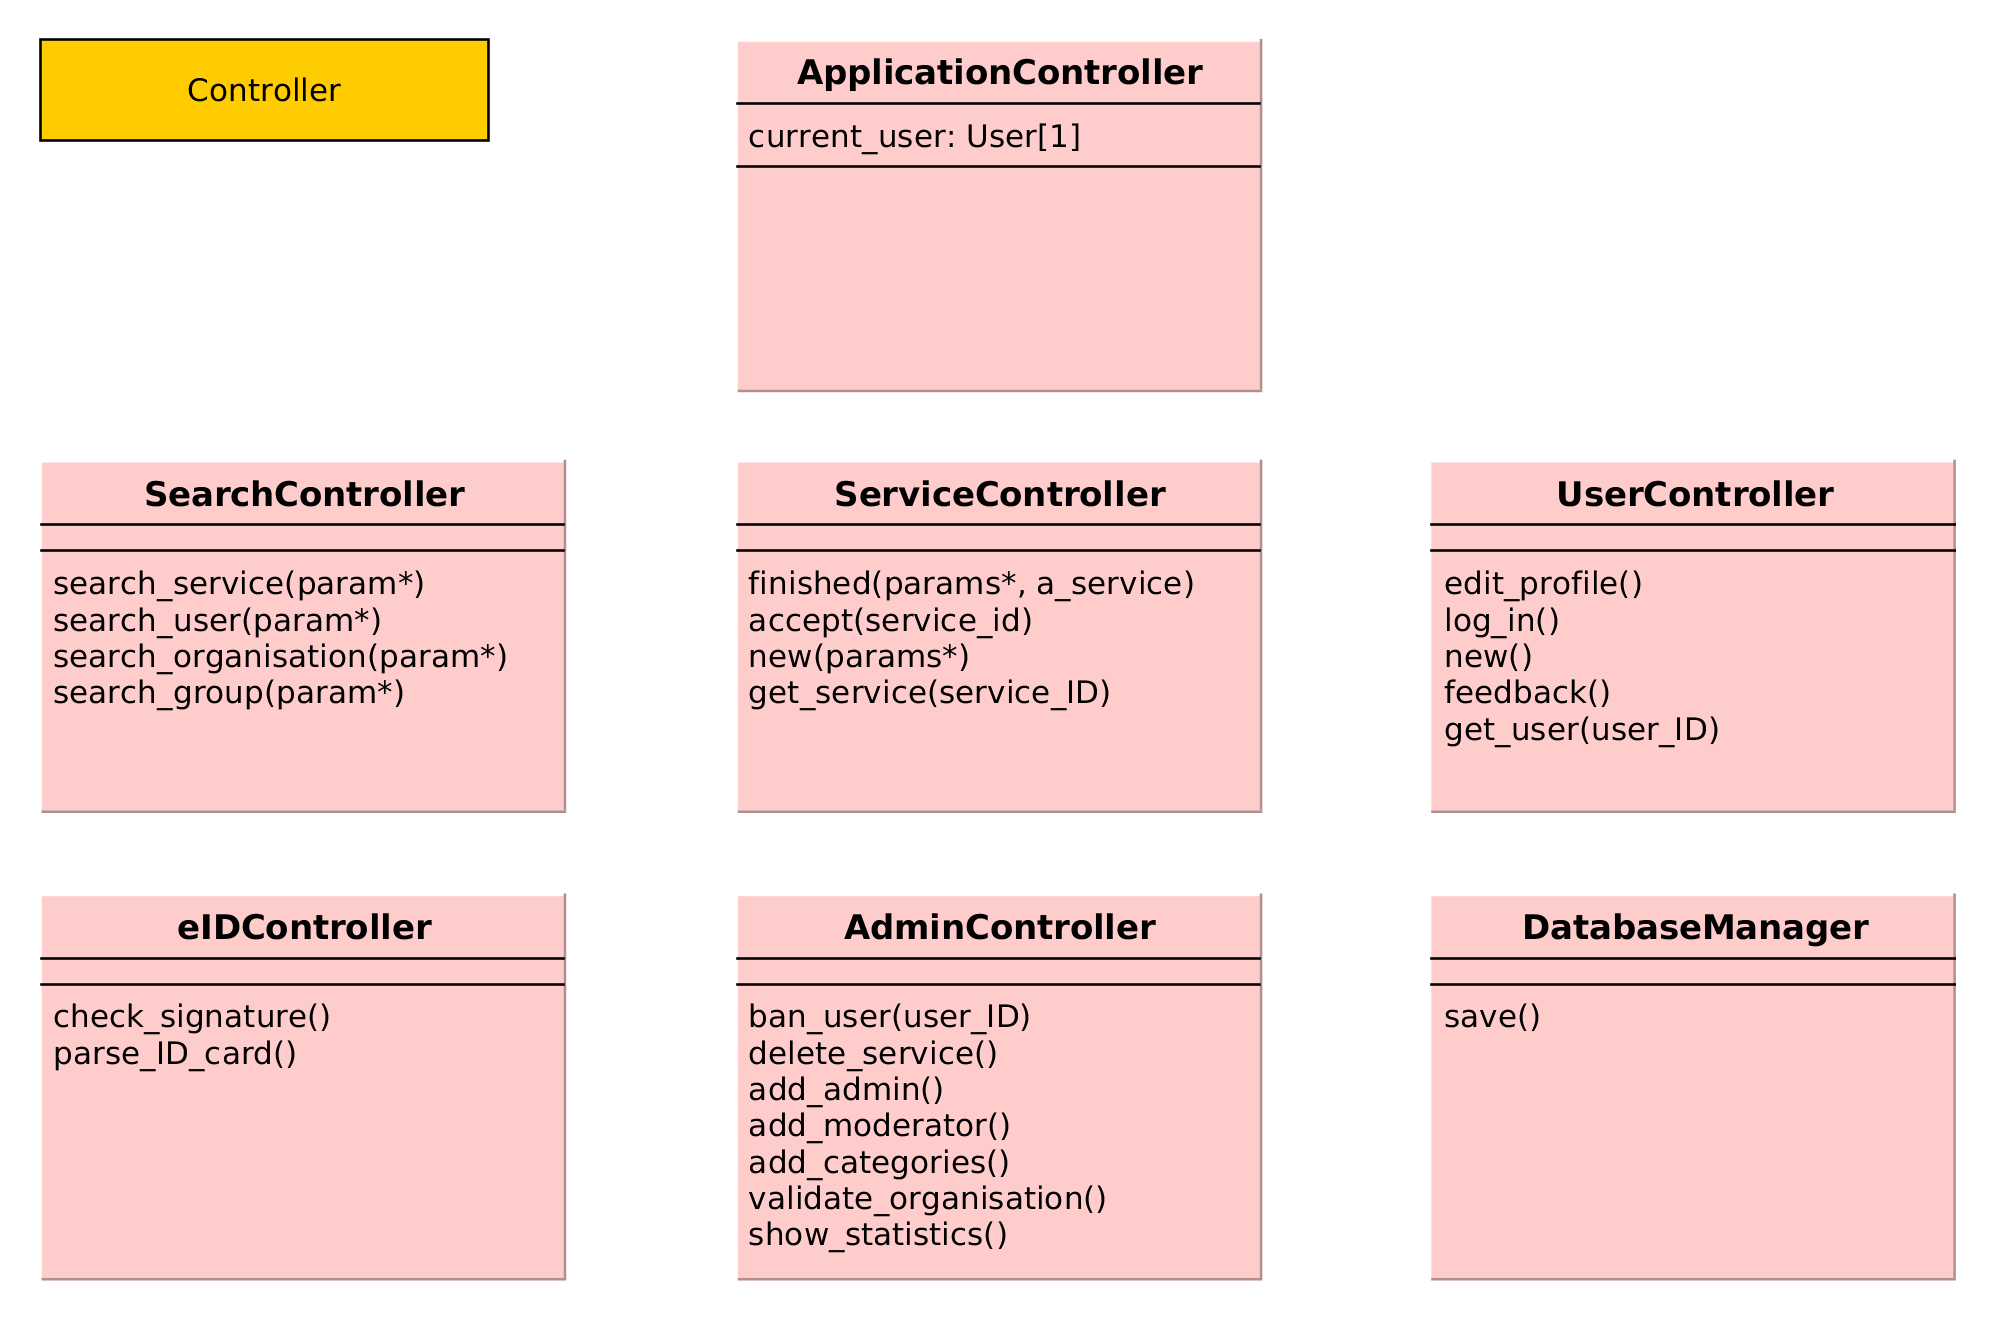
\includegraphics[width=.8\textwidth]{UML_Controller.png}
		\caption{Unified Modeling Language (UML): class diagram, controller.}
		\label{fig:uml_controller}
	\end{center}
\end{figure}

In an effort of completeness, we made a controller class diagram related to all methods and functions written in the sequence diagrams that are shown below. There are no relation between them because Rails manages these relations on his own. The application controller is the main one with most responsibilities. 

\subsection{Sequence diagrams}

\begin{figure}[!ht]
	\begin{center}
		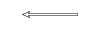
\includegraphics[scale=.5]{dubble_arrow.png} %% 75
		\caption{A double arrow is used to indicate an action of routing}
		\label{fig:darrow}
	\end{center}
\end{figure}
In the following diagrams, we decided to use the double arrow (like the one on figure \vref{fig:darrow}) to indicate an action of routing. It means that in the entry point of a diagram a user has been redirected to this page. Or at a moment of the diagram after some actions the user is redirect somewhere else on the website.

\texttt{current\_user} is a global variable which represents the user who is actually connected. The default value, when no user is connected, is \texttt{NULL}.

Another convention is \texttt{params*}. It represents all the parameters given by the form when we create an object like a user or a service.

\subsubsection{Log-in}

\begin{figure}[H]
	\begin{center}
		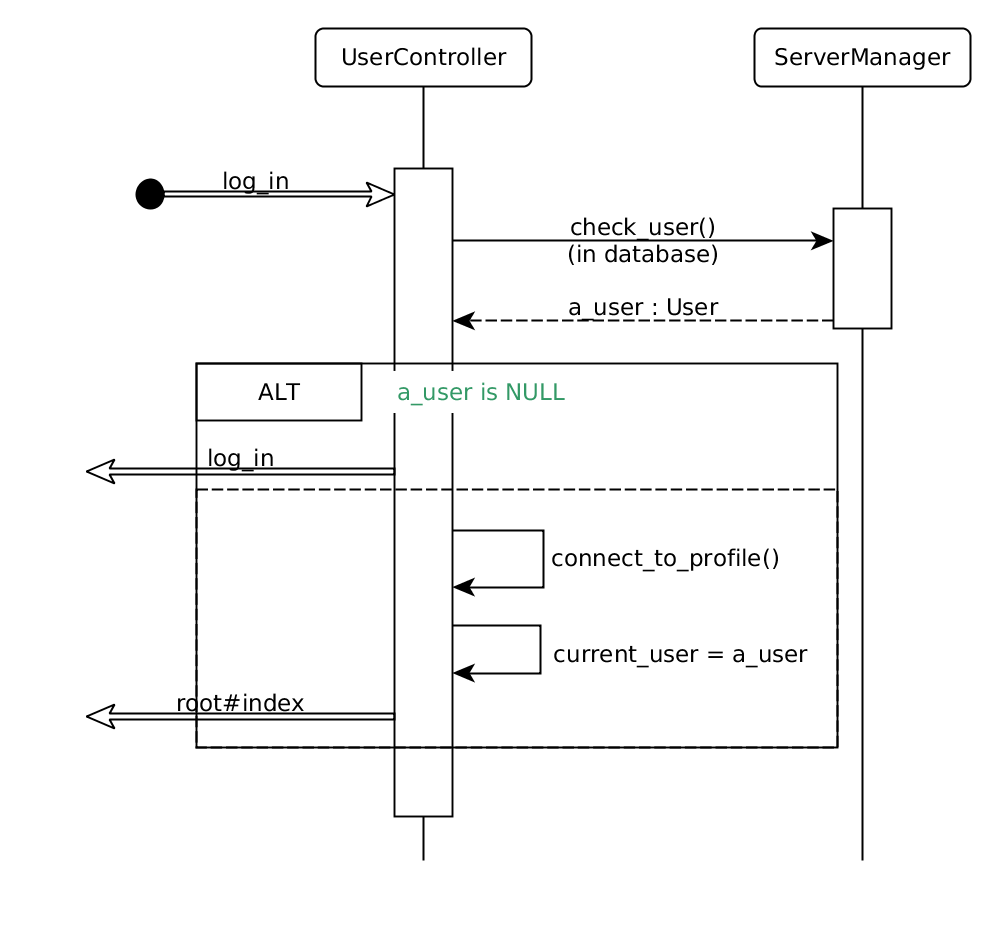
\includegraphics[width=.45\textwidth]{log_in.png} %% 70
		\caption{Sequence Diagram: Log-in}
		\label{fig:login}
	\end{center}
\end{figure}

This scheme modeles the action sequence when a user try to log in. As we can see, we check in
the database if this user exist. To do this we make a request that returns a \texttt{User} object. If
the user doesn't exist in the database, then this object is \texttt{NULL}. In this case,
we redirect the user to the log in page of the website ; otherwise, we connect to the profile and the current user is updated.

\subsubsection{User account creation}

\begin{figure}[H]
	\begin{center}
		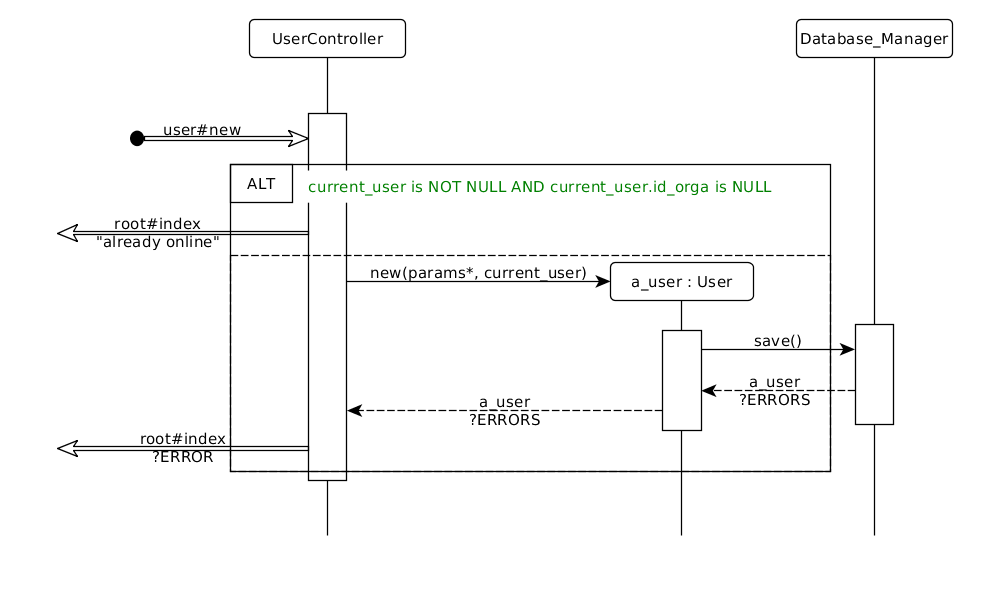
\includegraphics[width=.7\textwidth]{user_new.png} %% 100
		\caption{Sequence Diagram: User account creation}
		\label{fig:newuser}
	\end{center}
\end{figure}

To create a new user, we first have to check if the user is not already connected. If it is and if it's
not an organisation, then we redirect him to the root page because an already connected user cannot 
create a new account. In the case of an organisation, it is of course possible 
for it to create new users. Then, if no error occurs, we create a new \texttt{User} and we update its field \texttt{id\_orga}. This fields can contains \texttt{NULL} if the user creates his account on his own purpose or the id of the organisation that created for him. Then the user is added to the
database which send a response containing  possible error if the user already exists in the database.

\subsubsection{Search}

\begin{figure}[H]
	\begin{center}
		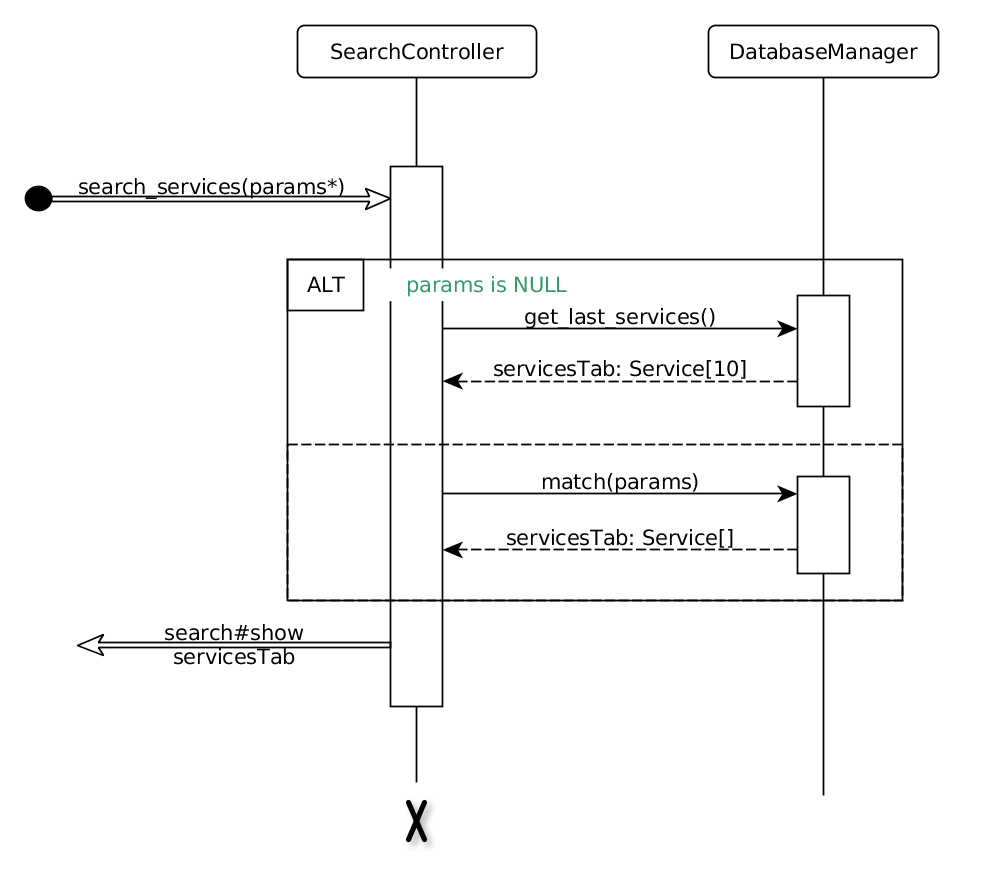
\includegraphics[width=.55\textwidth]{search_a_service.png} %% 80
		\caption{Sequence Diagram: Search a service}
		\label{fig:searchservice}
	\end{center}
\end{figure}

In this case, we show how the result of a search is proceeded. In the case where \texttt{params*} is \texttt{NULL}, we ask the database manager to return the ten last services (in a table \texttt{Service[]}) added to the platform ;
otherwise, we look at the database to do a match between the requested service represented by informations in the \texttt{params*} and the services that are available in the database. Finally the database manager sent an array of services containing either the "top ten" or the matching services.
Our extension is the advanced search.  To do that, we choose to change only the match method.  Then, the information in the \texttt{params*} change regarding the search we just made. 
\\If the client want to do more precise researches, we'll filter the results of the search on the client side. With this solution, we'll do less requests on the server.

\subsubsection{Service creation}

\begin{figure}[H]
	\begin{center}
		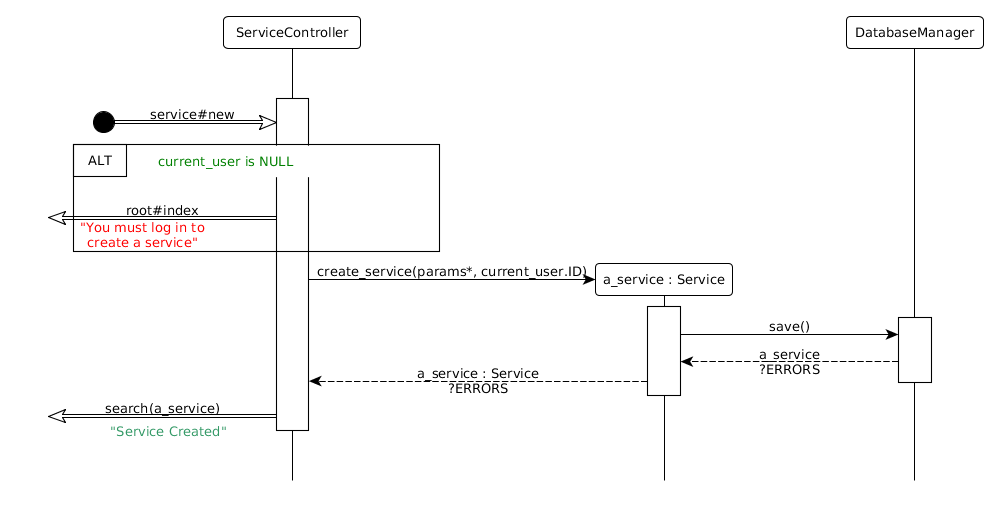
\includegraphics[width=.75\textwidth]{service_new.png} %% 100
		\caption{Sequence Diagram: Service creation}
		\label{fig:newservice}
	\end{center}
\end{figure}

We'll describe here the creation of a service. First, we check if the user is connected. If he is not, we redirect the user to the main page ; otherwise, we create a service object and we update its \texttt{id\_creator} field with 
the id of the current user. Then we save the service in the database. Finally, we redirect the user to a page displaying the result of a search with the newly created service.


\subsubsection{Service acceptance}
\begin{figure}[H]
	\begin{center}
		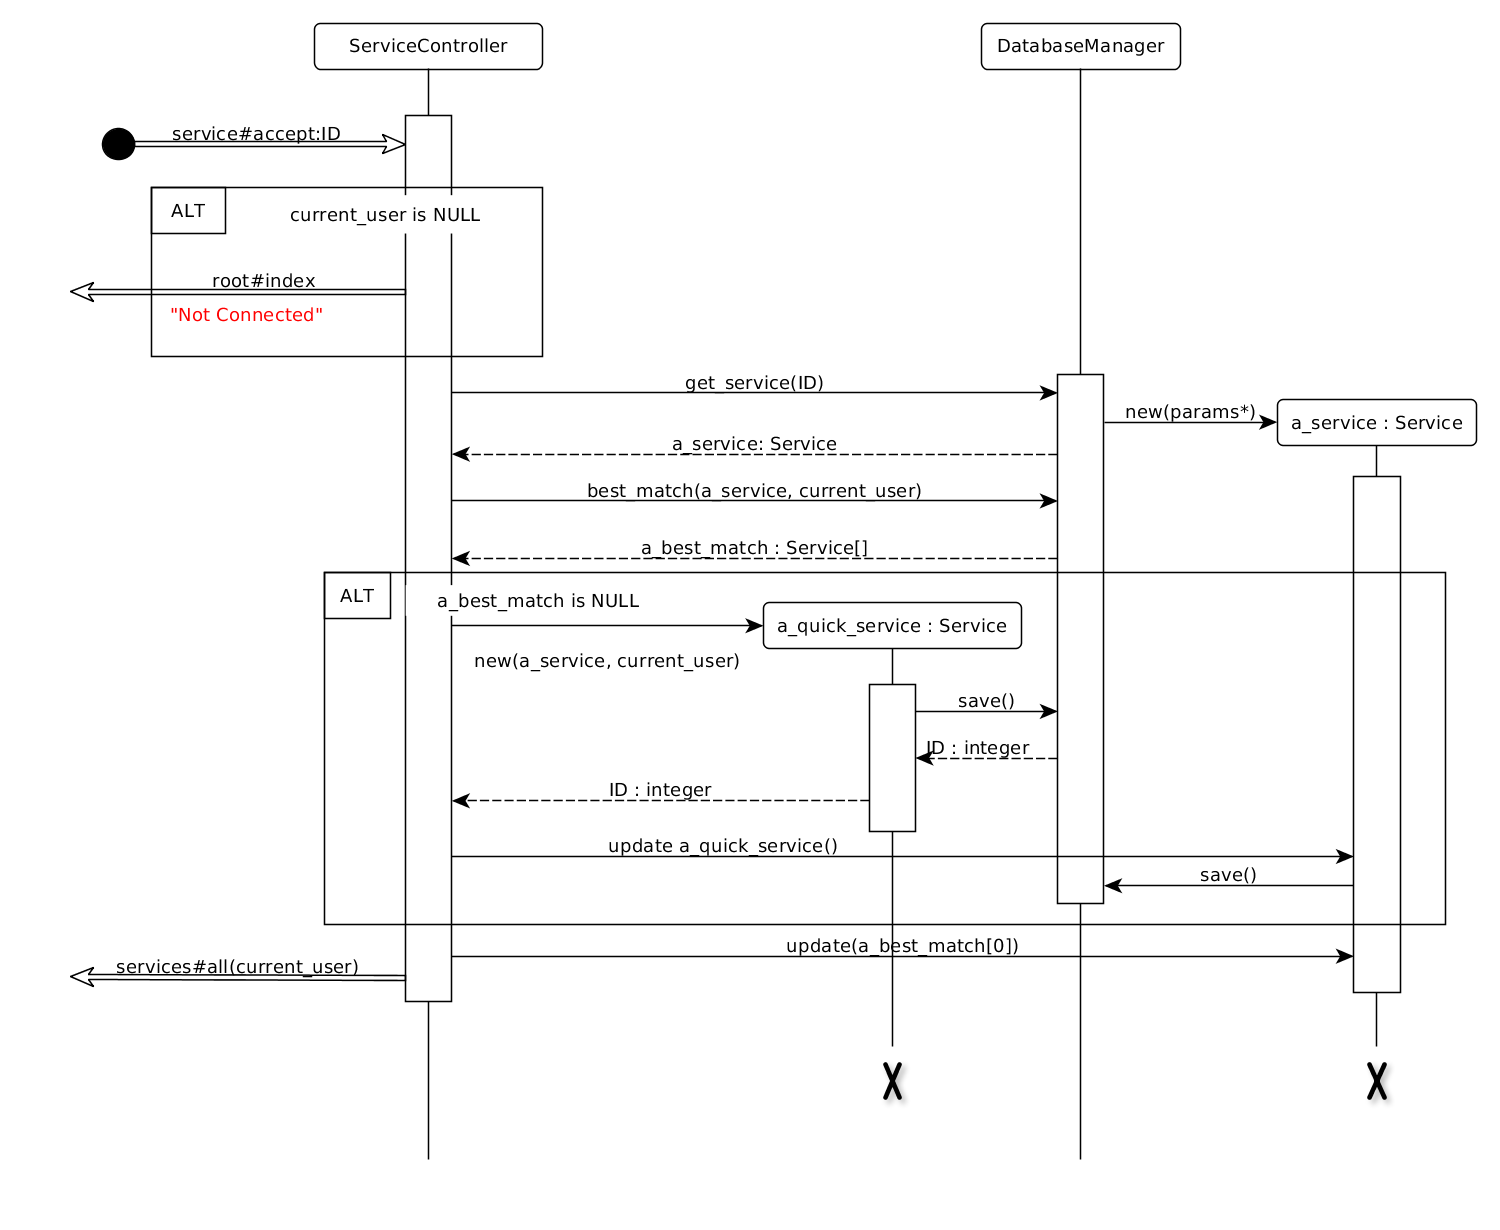
\includegraphics[width=.70\textwidth]{service_accepted.png} %% 95
		\caption{Sequence Diagram: Acceptance of an offer or a demand, visible in a bigger size in the appendix, figure \vref{fig:acceptService_big}}
		\label{fig:acceptService}
	\end{center}
\end{figure}

This scheme shows what happens when a service is accepted. First, we check if the user is connected.
If not, we redirect him to the home page. 
Then we proceed a \texttt{best\_match\_search} which returns all the services which match the request of the user.
If there are no result, we create a \texttt{Quick Service} which perfectly matches the user's expectation.

\subsubsection{End of service}
\begin{figure}[H]
	\begin{center}
		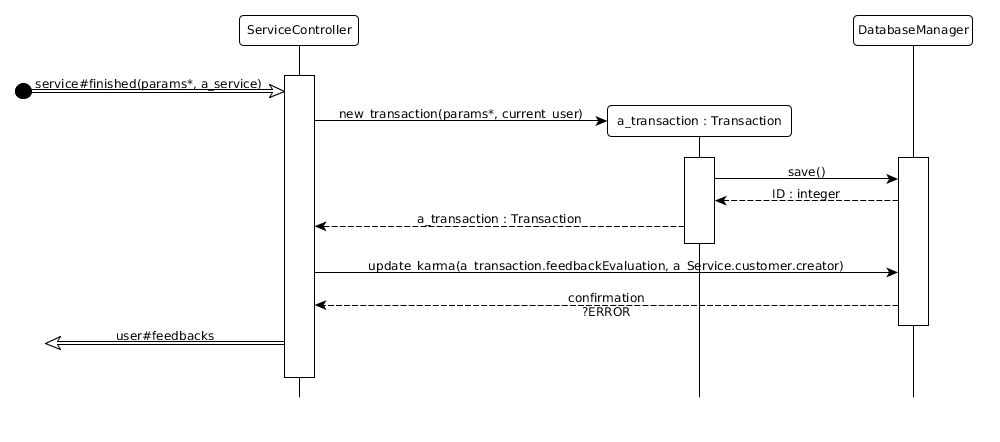
\includegraphics[width=.9\textwidth]{end_of_service.png}
		\caption{Sequence Diagram: End of a transaction}
		\label{fig:end_of_service}
	\end{center}
\end{figure}

When the creator and the customer have met and proceed the service, they can add a feedback for it.
When the creator or the customer do that, he fills a form (\texttt{params*} field on the figure below).  The route (\texttt{service\#finished}) is catching by the \texttt{ServiceController} and it creates a new transaction with the \texttt{params*} and the \texttt{current\_user}.
After that, we must update the karma of the other user that perform the service. The karma of the current user will be updated as well by the other
user.
Finally, we show the feedbacks page of the \texttt{current\_user}.

\subsubsection{Validation with the identity card}
\label{SEC:valid_ID}
\begin{figure}[H]
	\begin{center}
		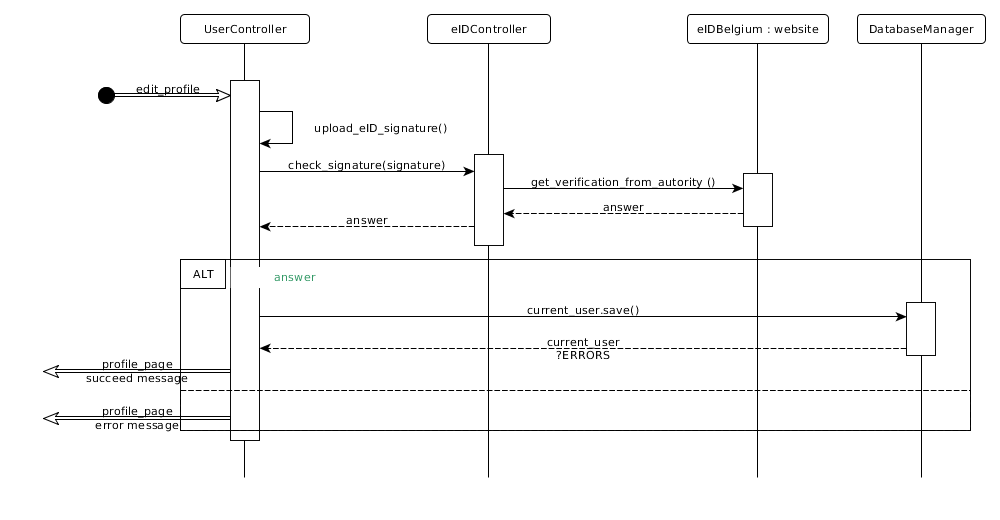
\includegraphics[width=1\textwidth]{check_ID.png}
		\caption{Sequence Diagram: Certifying a user by using the identity card}
		\label{fig:eID}
	\end{center}
\end{figure}

This diagram shows how the user can validate his account. After having received the signature, the \texttt{UserController} will use the \texttt{eIDController} to contact the authority in order to know if the signature is valid or not. If it is, the user is certified and we can save this information in the database.\\
At the end of this operation, the user is redirected to his profile page with a confirmation or an error message.\\
You can find this figure in bigger size in the appendix, figure \vref{fig:eID_big}.\\

To test the ID verification, the Belgium government provides a service\footnote{To learn more about that: \url{https://env.dev.eid.belgium.be/testkit.php}} that allow us to generate ID card.
As the ID verification functionality is an advanced properties. It will take lot of time to be developed, so we will implement it only if we have enough time.

\subsubsection{Ban from an Administrator}

\begin{figure}[H]
	\begin{center}
		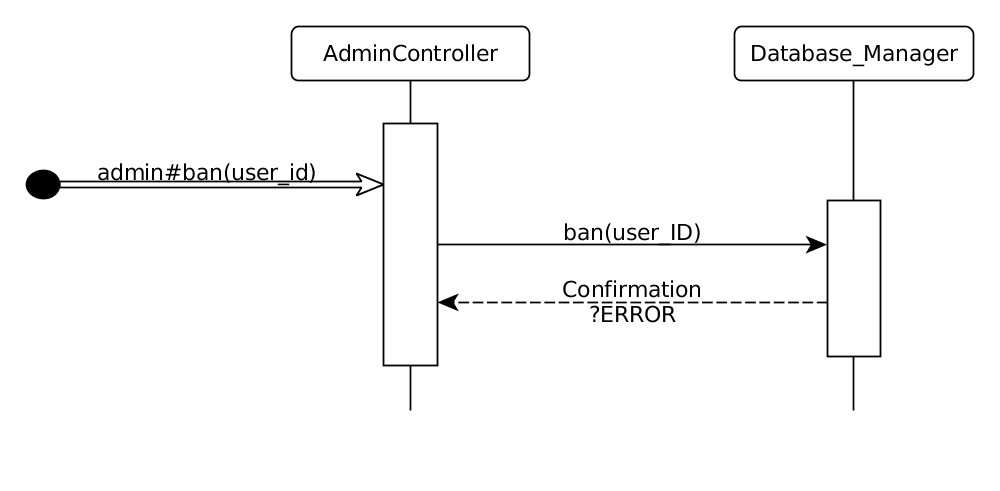
\includegraphics[width=.55\textwidth]{ban_user.png}
		\caption{Sequence Diagram: Ban a user from the website}
		\label{fig:ban}
	\end{center}
\end{figure}

In this scheme, we show one of the possible actions available to the administrator.
The method \texttt{ban(user\_id)} just check for the user corresponding to the id and edit his \texttt{inscription\_ok} in the database with the \texttt{False} value.


\subsection{Box Pointer Diagram}
 \begin{figure}[H]
	\begin{center}
		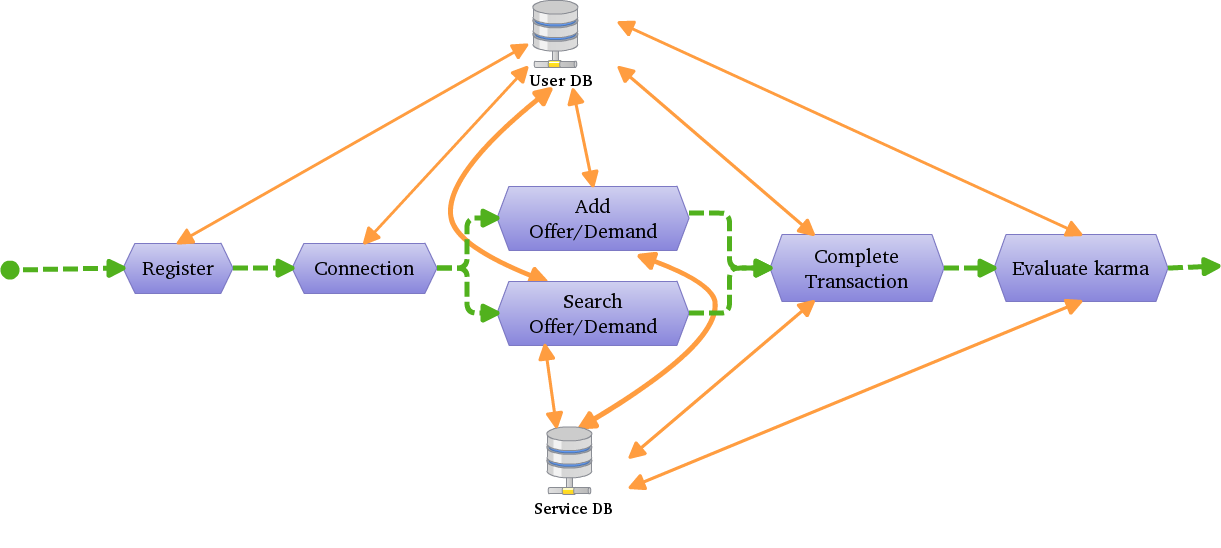
\includegraphics[width=.8\textwidth]{boxpointer.png}
		\caption{Box pointer diagram : Overall architecture}
		\label{fig:boxpointer}
	\end{center}
\end{figure}

In the previous report, we put this diagram to show a general overview of how the application should be used. In the feedback, we saw that it wasn't enough explained so we'll bring some additional informations about it. First, there are two databases shown but actually there will be only one in the real application. This was made to show which operation works with which part of the database. You can see this link with the orange arrows. The green arrows show a general flow of using the application in terms of time.
